
\section{Implementation}

In this section, we first describe the Wiki Link Data set we use for experiments.
Next, we present a micro benchmark to validate our investigation of entity approximation and compression.
We then discuss the implementation of the compression and approximation techniques over a large real-world
cross-document coreference corpus.

\subsection{Wiki Link Corpus}

The Wiki link corpus is the largest fully labeled cross-document coreference resolution data set to date~\cite{singh12:wiki-links}.
When downloaded, the data set contains 40 million mentions and almost three million entities --- it is a compressed 180 GBs of data.
The wiki link corpus was created by crawling pages across the web and extracting anchor tags that referenced Wikipedia articles.
Each page contains multiple multiple mentions of different types.
The Wikipedia articles act as the truth for each mention.


\subsection{Micro benchmark}
\label{sec:microbenchmark}
To increase our intuition of early stopping techniques we simulated the MCMC proposal processes. 
We hypothesis that there is a clear range values where performing the
baseline cluster sampling would be faster when compared to early stopping methods.
We arrange entity clusters of increasing time and we compute the time (in clock ticks)
each proposal takes to compute the arrangement of the clusters.
The data in the clusters are distributed uniformly and for this experiment each cluster point
was 5 dimensional.
For the baseline cluster score computation we used a pairwise calculated of the average cosine distance
with and without the mention.
To compute early stopping we set a confidence threshold to $0.8$ and the early
stopping code stopped computation when the error predation was under $20\%$.
There was no difference in the proposal choices between the baseline and the early sorting method. 

The simulations were developed in \texttt{GNU C++11} and compiled with \texttt{g++ -O3}. 
The CPU was an 8 core Intel i7 with 3.2 GHz and 12 GBs of Memory.
Each arrangement was run 5 times and results averages.



\paragraph{Early stopping or baseline.}
We first determine when early stopping approaches from proposal scoring is beneficial.
For this result we compare the base like proposal evaluator with a confidence-based scorer for varying entity sizes.
The result of this experiment is summarized in Figure~\ref{fig:clustering-v-early-stopping}.
On the x-axis is the number of mentions in the source and destination cluster is for each proposal. 
The y-axsis is the number of clock ticks on a log scale.

\begin{figure}
\centering
%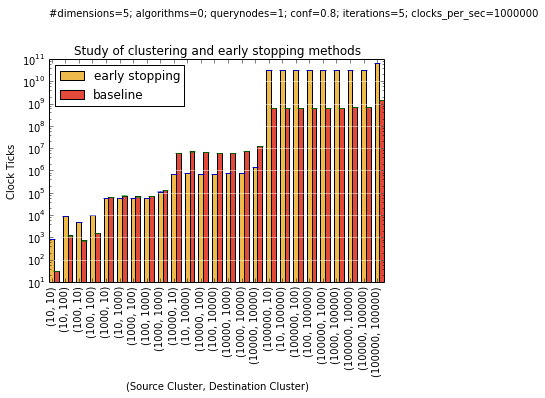
\includegraphics[width=\columnwidth, clip=true,trim=0cm 0cm 0cm 1.2cm]{media/clustering-v-early-stopping.png}
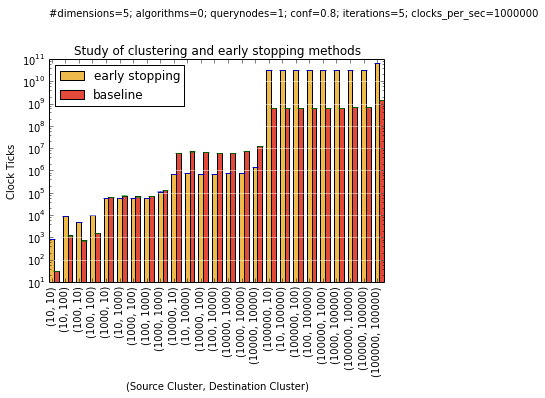
\includegraphics[width=\columnwidth, clip=true,trim=0cm 0cm 4cm 1.2cm]{media/clustering-v-early-stopping.png}
\caption{Comparison of baseline verses early stopping methods.}
\label{fig:clustering-v-early-stopping}
\end{figure}

We observe that for proposals with less than 100 and 1000 source and
destination mentions, the performance of the baseline proposer is better than
or almost equal to that of the more sorted early stopping method.
For proposals that contain an entity cluster with 10000 mentions
the early stopping method performs significantly better than the baseline method.

Surprisingly, the baseline proposals for for entities clusters containing $100 K$ mentions
performed over an order of magnitude better than the early stopping method.

The optimization found in predictable code paths make simple implementations
like the baseline method attractive for small cluster sizes and very large clusters sizes.
In addition, $82\%$ of the entities in the truthed Wiki links data sets are less
that 1000 mentions in size and $45\%$ of the entities contain less than 100
mentions.

The results of the micro benchmark suggests that different proposal estimation
techniques are useful at different times.
Note that for these techniques a small constant amount of book keeping space is required to perform early stopping.


\paragraph{Insertion vs Compressions Time.}
Compressing an entity is an expensive operation.
When compression and entity, this entity must be locked to prevent any concurrent access.
In order to choose the best times to compress an entity cluster in this 
micro benchmark we look at the time to compression entity of different cardinalities
and compare them to the time it takes to insert entities. 
Using a synthetic data set we generated entities of varying sizes and cardinality.
This experiment is shown in Figure~\ref{fig:compression-v-insertion}. 


\begin{figure}
\centering
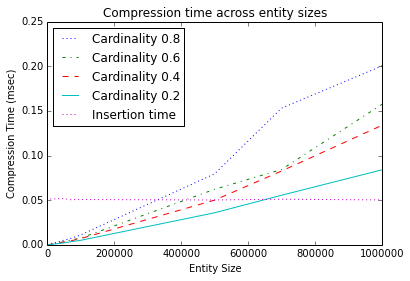
\includegraphics[width=\columnwidth]{media/compression-entitysize.png}
\caption{The time for compression for varying entity sizes and cardinalities.This is compared with line representing the time it take to make 100K insertions. }
\label{fig:compression-v-insertion}
\end{figure}

Cardinality number is a ratio of duplicates in the data set.
For example, Cardinality 0.8 means 8 of 10 items in the data set are duplicates.
The graph shows that in the time it take to compress entities of about 300K
the sampler could make 100K samples.
We can conclude from these result that compressing large entities is expensive
should only be done if the cluster is prohibitively large and not popular.

Cardinality estimation for millions of entities is a significant overhead.
Tracking cardinalities, in each entity, even using small probabilistic sketches such as Hyperloglog~\cite{flajolet2008hyperloglog}
become prohibitive at large sizes.
By the time an entities cardinality needs to be monitored for possible compression, that entity might as well be compressed.
We are continuing to look for lighter weight, cardinality estimators for millions of mentions.



